% #############################################################################
% This is Chapter 5
% !TEX root = ../main.tex
% #############################################################################
% Change the Name of the Chapter i the following line
\fancychapter{Exploring Parameter-Efficient Strategies in Transfer Learning for Children-Focused ASR Systems}
\label{chap:5}
\cleardoublepage

\section{Introduction}
The use of increasingly larger models coupled with the abundance of massive datasets is driving rapid advancements in many domains of machine learning, encompassing \ac{NLP} \cite{brown2020language} and computer vision \cite{ramesh2021zero}. In the context of \ac{ASR}, this trend of scalling up models is exemplified by state-of-the-art models such as Whisper \cite{radford2023robust} and HuBert \cite{hsu2021hubert}, where the number of parameters can exceeds 1 billion. Research has underscored the interconnected nature of the training dataset size and the number of model parameters, identifying them as mutual bottlenecks that influence the performances of machine learning models. This observation accentuates the significance of scaling these two dimensions in tandem for the development of more robust and effective \ac{ASR} models \cite{Kaplan2020ScalingLF}. Typically, to scalling up the model size a combination of an increased number of layers and an expansion of the model's hidden dimensions is used \cite{zheng22d_interspeech}.

However, the challenge arises when only a limited amount of data is available, making it challenging to train these large models from scratch, as highlighted by recent studies \cite{sri_end2end, gelin2021endtoend}. Hence, as discussed in the preceding chapter, transfer learning emerges as a well-established and effective paradigm to tackle to problematic of limited dataset. Nevertheless, despite its efficacy, we emphasised certain limitations that may potentially impede the performance of fine-tuning. Specifically, attempting to fine-tune these large models using a downstream dataset limited in size can be challenging. Indeed, in addition to be an expensive process, using small amount of data on such big model could potentially result in overfitting. This issue necessitates careful consideration, particularly in light of the recent evolution towards ever-growing pre-trained model sizes. Additionally, even following last chapter highlights where only specific parts of the model were fine-tuned, the different part of the model could be intricately linked to the overall model size. For example, \ac{FFN} modules usually represent substantial portion, around 70\% of the total number of parameters. This insight underscores the persistence of the challenge associated with model size, even when fine-tuning only specific components. Finally, TL on large amount of parameters is memory-storage-inefficient, especially when there is a need to store a replicas of the billion of parameters models for many different small tasks.

Consequently, there is a growing need for more \ac{PETL} as lightweight alternatives.
 Among the approaches introduced by the research community, residual Adapter modules stand out as the most popular and promising \cite{houlsby, pfeiffer}. Specifically tailored for Transformer-based systems, Adapters integrate a compact set of additional layers into a pre-trained source model. This design enables Adapters to enhance computational efficiency, resulting in faster training and addressing the challenge of catastrophic forgetting. Diverging from conventional transfer learning methods, where the source pre-trained model's weights are entirely replaced, Adapter-transfer maintains the integrity of the backbone model. Therefore, when the Adapter modules are removed, the initial pre-trained model remains unchanged. This preservation of the backbone model is a crucial advantage  as it offer increased flexibility. Furthermore, owing to their limited number of trainable parameters, Adapters demonstrate a decreased susceptibility to overfitting, thereby contributing to improved generalisation performance.

 In this chapter, our exploration is motivated by the promising characteristics of Adapters, and we will investigate their application in the specific context of children's \ac{ASR}. The study will encompass the examination of diverse Adapter configurations within both Transformer and Conformer architectures. Additionally, a novel proposition involves the introduction of a speaker-group-based Adapter using unsupervised cluster over speaker-embedddings.
The primary objective of this chapter is to address the overarching research question: \textit{Is it possible to develop an parameter-efficient automatic speech recognition model for children?} The investigation aims to unveil the potential for creating a model that optimally balances parameter efficiency and recognition accuracy. 

\section{Adapter tuning}

\begin{figure*}[t]
    \begin{center}
    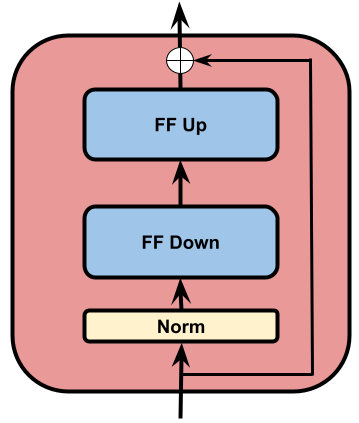
\includegraphics[scale=0.3]{imgs/Adapter_alone.png}
    \caption{Residual Adapter architecture}
    \label{fig:Adapter_architecture}
    \end{center}
    \end{figure*}


Adapters were initially introduced in the \ac{NLP} field to efficiently adapt large models, such as Transformers, using minimal amount of parameters for text classification \cite{houlsby}. As an alternative to full model fine-tuning, Adapter-transfer involves training an extra small number of task-specific parameters while keeping the original model frozen. This is done at each Transformer layer level by plugging them after the \ac{MHA} and \ac{FFN} modules, a setup often referred to as the \textit{Houlsby} configuration. Subsequently, \cite{pfeiffer} demonstrated that Adapters placed only after the \ac{FFN} modules were sufficient for achieving efficient performances, referred to as the \textit{Pfeiffer} configuration. Generally, Adapters employ a bottleneck architecture, consisting of a normalisation layer followed by a projection-down linear layer with a non-linear activation, and subsequently a projection-up linear layer. Finally, a residual connection is applied by summing the input of the Adapter with its output. The overall structure is illustrated in Figure \ref{fig:Adapter_architecture}. Research suggests that the hidden dimension, between the down and up projections, may not always benefit from a bottleneck structure, where $d_{hidden} < d_{model}$, and the optimal design may vary depending on the downstream task. In some tasks, an hidden dimension larger than the model size itself, in other words $d_{hidden} > d_{model}$, has been proven more effitive \cite{fan2022draft}.

Some of the main advantages of Adapters are their parameter efficiency and modularity. This efficiency is particularly interesting when working with large pre-trained models, while the modularity is valuable when a large number of tasks need to be trained.
Mathematically, the structure of an Adapter can be expressed as follows:

\begin{equation}
    adapter(x) = x + (W_{up}(f(W_{down}g(x)+b_{down})))+ b_{up})
\end{equation}
Where $W_{down}$ and $W_{up}$ denote the weights of the projection-down and projection-up linear layers, and $b_{down}$ and $b_{up}$ represent the corresponding biases. The function $f(\cdot)$ is a non-linear activation, while $g(\cdot)$ a layer normalisation or identity function. Finally, $x$ corresponds the input given to the Adapter.

In terms of computation, Adapters offer the advantage of faster training, given that they update fewer parameters compared to fully fine-tuning models. However, there might be a slight processing delay during inference due to the addition of extra parameters introduced by the Adapters, this difference is generally minimal and can be well-managed \cite{ruckle2020adapterdrop}.

% Adapter ASR
Adapter-transfer has gained increased attention in the context of \ac{ASR} tasks \cite{cappellazzo2023parameter,chen2023efficient,10095837}, particularly owing to its modular nature, which has proven advantageous in the context of multi-lingual \ac{ASR} \cite{kannan2019large, hou2021exploiting, kulkarni2023adapting}. In these studies, distinct Adapters were trained for each language, contributing to enhanced performance compared to a monolingual model and mitigating certain challenges associated with transfer learning, such as overfitting. This modular approach provides a tailored solution, as each Adapter designed for a specific language can effectively capture the diverse acoustic characteristics unique to that language.

In addition, researchers have explored the use of Adapters in the context of \ac{SSL}. In \ac{SSL}, larger model are typically employed to capture a wide range of information from speech for application in a broad spectrum of tasks \cite{thomas2022efficient, fan2022draft}. However, the computational cost and scalability to multiple tasks can pose a challenge. Notably, once the model is fine-tuned for a specific task, the entire model is fixed for that task, and re-loading and re-training the base model are necessary for transferring to a different task. Therefore, the use of Adapters has proven effective in addressing these challenges by providing a modular and parameter-efficient task-specific adaptation.

Additionally, the effectiveness of Adapters has been demonstrated in addressing challenges related to low-resource and atypical speech recognition scenarios \cite{tomanek2021residual}

Finally, the effectiveness of Adapters has also been demonstrated in addressing challenges related to low-resource and atypical speech recognition scenarios \cite{tomanek2021residual}. In such scenarios, similarly to children's speech, there is limited availability of labeled data and atypical speech characteristics. As a result, Adapters provide a valuable solution by efficiently adapting large pre-trained models to these challenging tasks. 

% Adapter children
However, the application of Adapters in the context of children's \ac{ASR} has received limited attention, with only one notable study by \cite{fan2022draft}. In this study, the authors proposed integrating and training Adapters within \ac{SSL} models, followed by fine-tuning the entire model, including the Adapter weights, for better modeling of children's speech. This represents a pioneering effort to leverage Adapters for adapting large-scale models to the unique characteristics of children's speech.

\section{Investigating Adapters for Children's ASR}

\begin{figure*}[t]
    \begin{center}
    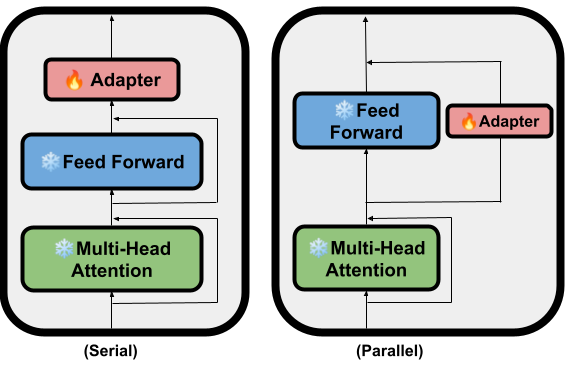
\includegraphics[scale=0.27]{imgs/Adapter_Transformer.png}
    \caption{Transformer block with various residual adapter configurations. Normalisation layers are not display in this figure}
    \label{fig:transformer_config}
    \end{center}
\end{figure*}
\begin{figure*}[t]
    \begin{center}
    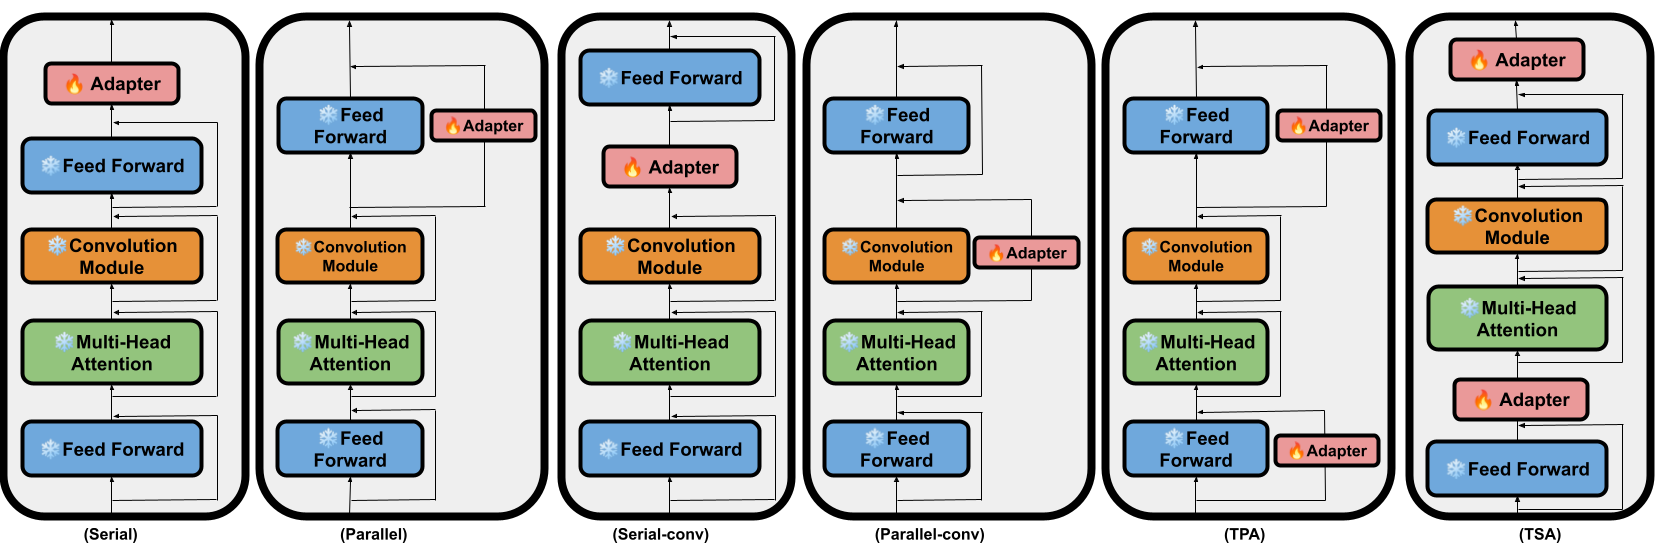
\includegraphics[scale=0.27]{imgs/Adapter_conformer.png}
    \caption{Conformer block with various residual Adapter configurations. Normalisation layers are not display in this figure}
    \label{fig:conformer_config}
    \end{center}
\end{figure*}

In this section, we delve into the application of Adapter-transfer as \ac{PETL} for both Transformer and Conformer architectures in the domain of children's \ac{ASR}. Building upon our findings from the previous chapter, where we identified the \ac{FFN} modules as the most relevant component to fine-tuning in a Transformer-based model, we opt to leverage Adapters for modifying the output of these \ac{FFN} modules. Additionally, considering our results that underscore the significance of fine-tuning the Encoder, our primary emphasis will be on investigating the implementation of Adapters within the Encoder. Specifically, for the Transformer architecture, we investigate two integration methods: parallel and serial placement with the \ac{FFN} component. Such configurations were used in prior work \cite{he2022towards} and are depicted in Figure \ref{fig:transformer_config}.

In the case of the Conformer architecture, we explore six distinct Adapter configurations, as illustrated in Figure \ref{fig:conformer_config}. The initial two configurations mirror our Transformer investigation, involving both parallel and serial placements, either after or in parallel with the second \ac{FFN} layer \cite{chen2023efficient}. Additionally, we assess a configuration that introduces an Adapter following the convolution module, denoted as the \textit{serial-conv} setup used in \cite{10095837}. Notably, although the \ac{FFN} component has been identified as the most crucial for fine-tuning, promising results have also been observed by fine-tuning the convolution modules \cite{chen2023efficient}. Furthermore, \cite{chen2023efficient} introduces two variants of the parallel setup: \textit{parallel-conv} where the Adapter operates in parallel with the convolution module, and the \textit{\ac{TPA}} configuration where two Adapters are placed in parallel with both \ac{FFN} modules in each Conformer layer. This comprehensive exploration of Adapter configurations within both architectures aims to discern the most effective adaptation strategies for children's speech in the context of \ac{ASR}. 


In the case of serial configurations, the integration of Adapter information is performed with the preceding component denoted as $P$. The specific component $P$ varies depending on the configuration and can be either \ac{FFN} or convolution modules. This integration is realised through the following process:

\begin{equation}
    output =  Adapter(P(x))
\end{equation}

where $x$ represents the input of component $P$.

For parallel configurations, the integration process varies slightly. In this scenario, the adapter's output is combined with the output of component $P$ as follows:

\begin{equation}
    output = x + 0.5 \cdot P(x) + (Adapter(x) - x)
\end{equation}

where $x$ is the input of component $P$.

To comprehensively explore all feasible configurations, we introduce two novel setups. The first one is referred to as \textit{\ac{TSA}} where two Adapters are sequentially positioned after each \ac{FFN} component in all layers. The second configuration combines \ac{TPA} and \ac{TSA}, resulting in the integration of four Adapter modules both in parallel and serially at the two \ac{FFN} modules level. 


Moreover, we consider three distinct configurations where Adapters are placed in the Decoder. It is important to note that in the Conformer architecture, the Decoder is a regular Transformer. Therefore, we evaluate the \textit{Serial} and \textit{Parallel} setups. Subsequently, we investigate the combination of the most effective Encoder Adapter configuration with both Decoder configurations. To the best of our knowledge, there is no prior research that formally investigates the influence of Adapters within an \ac{ASR} Decoder. 

Finally, motivated by the observed strong correlation between children's speech variability and age, we explore the possibility of training specialised Adapters. However, considering the high inter-speaker variabilities in children's speech, using age directly may not effectively capture children with similar acoustic characteristics. Additionally, in many children's speech datasets, precise age information is often not provided. To address this, we partition the training dataset into groups of speakers with similar acoustic characteristics based on unsupervised clustering.
In practice, we apply a k-means clustering algorithm on the x-vector representation \cite{snyder2018x} of all training utterances. Subsequently, distinct Adapters are trained for each speaker cluster separately. During the testing phase, the closest clusters of group of speaker is determined for each test utterance, and the corresponding Adapters specific to that group are employed for decoding.

The primary objective of these experiments is to investigate whether Adapters trained on comparable speech characteristics yield improvements over a general Adapter on the entire training set. Indeed,
% No work fully compared Adapter vs Conformer in Children speech
children's speech is inherently atypical and displays a significant degree of variability, making it imperative to assess the efficacy of existing methods. In prior work, different configurations were employed resulting in a lack of standardised evaluation.

\section{Implementation details}

All experiments were performed using the SpeechBrain toolkit \cite{speechbrain}. We used  12 Transformer or Conformer layers for the Encoder, for the Transformer and Conformer model respectively, and 6 Transformer layers for the Decoder, all with dimensions 512. These models have been pre-trained using the LibriSpeech dataset \cite{librispeech} and are publicly available\footnote{https://huggingface.co/speechbrain/ASR-transformer-transformerlm-librispeech} \footnote{https://huggingface.co/speechbrain/ASR-conformer-transformerlm-librispeech}. Furthermore, for all of our experiments, we used the same Transformer language model, trained on 10 million words 
%CAMERA-READY (Add Information about the Language model training)
on the LibriSpeech transcriptions.
The Adapter architecture consists of a  first linear layer projection to dimension 512 with a ReLu activation, followed by another linear layer projection to dimension 512 with a residual connection of the Adapter input. For all Adapters, in the initialisation process, we set $W_{down}$ to all zeros, and $W_{up}$, $b_{down}$, $b_{up}$ are initialised using Xavier initialisation \cite{glorot2010understanding}.


The use of a hidden-dimension size equal to the model size (instead of a bottleneck) was motivated by previous research exploring hidden-dimension size, that consistently demonstrated that larger dimensions tend to yield improved performance scores \cite{chen2023efficient}.
All models were trained for 30 epochs, with a learning rate of $8\cdot10^{-4}$ for Adapters experiments and of $8\cdot10^{-5}$ for fine-tuning the entire model.
For the clustering experiments, we use the k-means clustering algorithm on the speaker-embedding of each utterance. The speaker embeddings were extracted using a publicly pre-trained ECAPA-TDNN model, trained on adult speech\footnote{https://huggingface.co/speechbrain/spkrec-ecapa-voxceleb}.

\section{Results}
\label{sec:results}

\subsection{Configurations}
\begin{table}[t]
\caption{Results of the different Adapters configurations in both Transformer and Conformer.}
\begin{center}    
\begin{tabular}{ccc}
\hline
 Method & WER $\downarrow$     & Trained params    \\ \hline \hline
\multicolumn{3}{c}{Transformer} \\ \hline
\multicolumn{1}{l}{\textit{Frozen}} & 25.04\%   & - \\
\multicolumn{1}{l}{\textit{Full fine-tuning}} & 12.99\% & 71.5M \\ \hline
\multicolumn{1}{l}{Serial}  &   12.78\% & 6.3M  \\ 
\multicolumn{1}{l}{Parallel}  &     \textbf{12.62\%} & 6.3M  \\ \hline\hline
\multicolumn{3}{c}{Conformer} \\ \hline
\multicolumn{1}{l}{\textit{Frozen}} & 21.75\%   & - \\ 
\multicolumn{1}{l}{\textit{Full fine-tuning}} & 12.28\% & 109.1M \\ \hline
\multicolumn{1}{l}{Serial}  &   11.76\% & 6.3M  \\ %11.84 
\multicolumn{1}{l}{Serial-Conv} & 11.78\%     & 6.3M  \\
\multicolumn{1}{l}{Parallel}    & 11.72\% & 6.3M  \\ % 11.88 
\multicolumn{1}{l}{Parallel-conv} & 11.79\%      & 6.3M  \\ %\hline
\multicolumn{1}{l}{TPA} & \textbf{11.58\%}     & 12.6M  \\ %11.85
\multicolumn{1}{l}{TSA} & 11.75\%     & 12.6M  \\ \hline %11.72
\multicolumn{1}{l}{Serial (Decoder)} & 18.09\%     & 3.2M  \\ 
\multicolumn{1}{l}{Parallel (Decoder)} &17.76\%     & 3.2M  \\ \hline
%\multicolumn{1}{l}{TPA + Serial (Decoder)} & 00.00(T)\%     & 15.8M  \\
%\multicolumn{1}{l}{TPA + Serial (Decoder)} & 11.68\%     & 15.8M  \\ 
\multicolumn{1}{l}{TPA + Parallel (Decoder)} & \textbf{11.47\%}     & 15.8M  \\ \hline

\end{tabular}
\end{center}

\label{tab:res}
\end{table}

In this section, we present a comprehensive evaluation of Adapter configurations applied to both Transformer and Conformer models, assessing their performance based on \ac{WER}, as presented in Table \ref{tab:res}.  First, we assess 
%CAMERA-READY ( remove this to make more clear that frozen is no-finetune and without adapters)
%Adapter configurations in 
the Transformer model when no fine-tuning was applied (\textit{Frozen}), resulting in a \ac{WER} of 25.04\%. Conversely, \textit{Full Fine-Tuning} involved complete fine-tuning of the entire model,
%CAMERA-READY (Make more clear that this is our baseline)
working as our baseline system
, reducing the \ac{WER} significantly to 12.99\%, at the expense of 71.5 million trainable parameters.
Turning to the Adapter setups, we investigate the \textit{Serial} and \textit{Parallel} configurations, both equipped with 6.3 million trainable parameters. The \textit{Parallel} emerged as the best configuration, achieving the lowest \ac{WER} of 12.62\% compared to 12.78\% for the \textit{Serial}. These results underscore the effectiveness of Adapter configurations within the Transformer architecture, as they both perform slightly better than the full-finetuning.

Next, we investigated the Conformer model, we once again explored \textit{Frozen} and \textit{Full Fine-Tuning}. In \textit{Frozen} the pre-trained model remained untouched, yielding a \ac{WER} of 21.75\%. The Full fine-tuning, in a similar way as the Transformer, led to enhanced performance, reducing the \ac{WER} to 12.28\% with a total of 109.1 million trainable parameters. We can observe that given the same pre-training dataset, the Conformer architecture outperforms the regular Transformers. Within the set of Adapter configurations, \textit{Serial} achieved a \ac{WER} of 11.76\%, while \textit{Parallel} demonstrated slightly better performance with a \ac{WER} of 11.72\%. These results indicated that \textit{Parallel} Adapters were more effective in improving \ac{WER} in the Conformer model. When Adapters are placed after the convolution layer, with the \textit{Serial-conv} and \textit{Parallel-conv} configuration, both slightly under-perform compared to Adapters placed after the second \ac{FFN} component with respective scores of 11.78\% and 11.79\%. Finally, we evaluated the \textit{\ac{TPA}}and \textit{\ac{TSA}} configurations. The \textit{\ac{TPA}} configuration emerged as the most promising, with a very remarkable \ac{WER} of 11.58\% using 12.6 million trainable parameters, while \textit{\ac{TSA}} achieved a \ac{WER} of 11.75\%, which is slightly under-performing compared to the \textit{\ac{TPA}}configuration.

In addition, we evaluated the use of  Adapters in the Decoder. As the Decoder of the Conformer architecture is a regular Transformer, we only evaluate the \textit{Serial} and \textit{Parallel} setup, which respectively reached 18.09\%  and 17.76\% \ac{WER} with 3.2 million parameters. Results showed that Adapters are more relevant when plugged into the Encoder. It confirms that acoustic variability plays a critical role in the degradation of children's \ac{ASR} performance. Finally, combining \textit{\ac{TPA}} in the Encoder layers with \textit{Parallel} Adapters in the Decoder outperforms Adapters in the Encoder only, with 11.47\% \ac{WER}. Consequently, this configuration stands as the most effective model. 

%statistical tests
We performed statistical tests (Matched Pairs Sentence-Segment Word Error) across all Adapter setups in comparison to the full fine-tuning configuration using SCTK, the NIST Scoring Toolkit \footnote{https://github.com/usnistgov/SCTK/tree/master}. 
The results reveal that, in all scenarios, the \textit{p}-value is less than or equal to 0.001. This observation denotes statistical significance, indicating evidence against the null hypothesis. 

These results collectively illustrate the versatility and effectiveness of different Adapter configurations within the Transformer and  Conformer model for the children's \ac{ASR} task. \textit{\ac{TPA}} Adapters in the Encoder combined with \textit{Parallel} Adapters in the Decoder showcased outstanding performance, highlighting their potential as a fine-tuning replacement in large model children \ac{ASR} scenarios.

\subsection{Effect of the Adapters hidden dimension}
\begin{figure}
    \begin{center}
    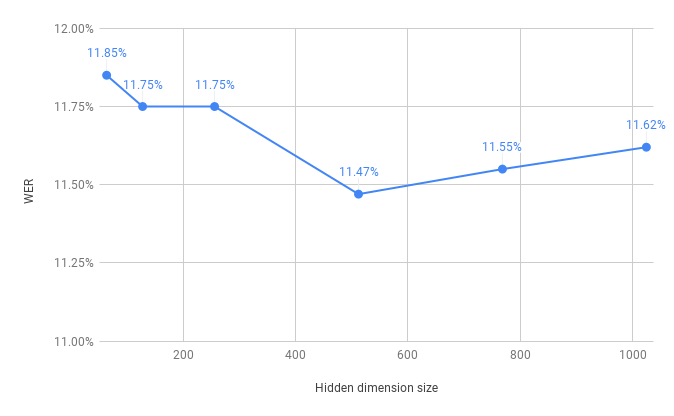
\includegraphics[scale=0.5]{imgs/HiddenDimEXP.png}
    \caption{Experimental Adapter transfer using different hidden dimension size within the Conformer architecture }
    \label{fig:HiddenDim}    
\end{center}
    
\end{figure}

In this section, our goal is to investigate the impact of varying the Adapter's hidden dimension $d_{hidden}$ on the performance of the model. While our previous experiments used a fixed hidden dimension equal to the hidden dimension of the Transformer and Conformer model, $d_{model} =  d_{hidden} = 512$. Here, we will explore different hidden dimension values within the Conformer architecture, specifically employing the \textit{\ac{TPA}} in the Encoder-only configuration. This investigation evaluate how variations in the hidden dimension may influence the performance of the Adapter transfer, providing valuable insights into the parameter tuning process for Adapter modules.

In Figure \ref{fig:HiddenDim}, the \ac{WER} performances of the Adapter transfer are presented in relation to the hidden dimension size ($d_{hidden}$). Notably, a delicate balance is observed, emphasising the importance of choosing an optimal hidden dimension size. Configurations with dimensions that are either too small or too large result in a degradation of overall performance. The best-performing configuration aligns with the choices made in all previous experiments, with $d_{hidden} = d_{model} = 512$. This observation supports the hypothesis that the parallel Adapter functions as an extension of the key-value memory of the \ac{FFN}. Opting for an extremely large hidden dimension makes training more complex due to the large amount of parameters, while an excessively small size drastically limits the potential information learned in the Adapters. 

\subsection{Unsupervised clustering for grouped-speaker Adapters}

In this section, we present the outcomes of our clustering approach, as summarised in Table \ref{tab:res_clusters}. The investigation focused on the influence of varying the number of cluster on the \ac{ASR} performance, ranging from 1 to 4 clusters, using the \textit{\ac{TPA}} configuration in an Encoder-only setup. First, when the data remained unclustered (one cluster), the \ac{ASR} system exhibited a 
\ac{WER} of 11.58\%. Notably, the two-cluster configuration outperformed the other setups, achieving a superior performance with a \ac{WER} of 11.50\%. This result suggests that partitioning the data into two distinct clusters allows the different Adapters to more effectively capture underlying patterns intricately linked to their respective clusters, consequently enhancing the recognition scores.
Furthermore, we explored the impact of increasing the number of clusters to three and four, revealing only marginal differences in performance. Specifically, the three-cluster configuration yielded a \ac{WER} of 11.57\%, and the four-cluster configuration resulted in a \ac{WER} of 11.51\%. These findings underscore the role of data clustering in children's \ac{ASR} systems by grouping shared speaker characteristics in different clusters.

In summary, our investigation underscores the significance of data clustering in children's \ac{ASR} systems. The optimal performance was achieved with a two-cluster configuration, suggesting that this approach enables the Adapters to capture cluster-specific patterns effectively. The marginal differences observed with three and four clusters highlight a potential saturation point where further partitioning offers diminishing returns in terms of \ac{ASR} performance improvement. It is worth noting that, in this experiment, the amount of available training data for Adapters varies due to clustering. A more comprehensive exploration of the impact of training hours on Adapters will be presented in Section \ref{sec:hours_PETL}. This will provide a more detailed analysis of how different training durations affect the performance of Adapters in varying conditions, offering insights into their adaptability and effectiveness in diverse scenarios.

\begin{table}[t]
    \begin{center}    
    \begin{tabular}{cc}
    \hline
      \# of clusters & Average WER $\downarrow$    \\ \hline
    \multicolumn{1}{c}{1} & 11.58\%  \\% OR 11.70%  If we consider 40 epochs instead of 30 here
    \multicolumn{1}{c}{2} & \textbf{11.50\%}  \\
    \multicolumn{1}{c}{3} & 11.57\%  \\
    \multicolumn{1}{c}{4} & 11.51\%  \\ \hline 
    \end{tabular}
    \end{center}
    \caption{Results of the unsupervised clustered Adapters approach.}
    \label{tab:res_clusters}
    \end{table}
    
\section{Summary and discussion}
% Summary
In this chapter, our exploration centered around investigating the viability of Adapter transfer in the context of children's \ac{ASR}. We answer the following research question \textit{Is it possible to develop an parameter-efficient automatic speech recognition model for children?} by a positive answer. Our study demonstrated the efficacy of efficiently adapting the model using Adapter modules, showcasing improved \ac{WER} performances compared to full-model fine-tuning, all while utilising only around 10\% of the parameters required in the traditional transfer learning configuration. Among the diverse configurations examined in this chapter, the Parallel Adapter and its extension, the \ac{TPA}, emerged as the most effective choices for the Transformer and Conformer architectures, respectively. This parallel Adapter can be perceived as an extension of the key-value memory that represent the \ac{FFN} modules, showcasing its potential for capturing essential children information in a more parameter-efficient manner.

Expanding upon our findings, we proposed to incorporate an unsupervised clustering on the speaker embeddings extracted the different utterances to the Adapter transfer procedure. This strategic separation aimed to facilitate the training of specific Adapters for each cluster, offering a more personalised adaptation without requiring detailed metadata about the speaker, such as their age. Our results demonstrated that leveraging these clusters could further enhance the overall performances, paving the way for the application of Adapters in personalised \ac{ASR} systems.

% Discussion
% Mention that this open the way for other used, such as reducing the domain mismatch
The feasibility of Adapter transfer in the domain of children's speech opens up new avenues for advancing children's \ac{ASR}. Our findings indicate that Adapters effectively bridge the gap between source and target domains, while preserving the pre-trained models and the knowledge it contains. This promising result paves the way for further research. In the upcoming chapter, we will explore the application of Adapters in the realm of \text{TTS} data augmentation. This extension of our research seeks to leverage the capabilities of Adapters for reducing the gap between real and synthetic children speech.
% Also mention that we will investigate other PETL approaches
In addition to presenting the Adapter module in this chapter, it is worth noting that a new variety of \ac{PETL} approaches exist in the literature, showcasing their effectiveness in tasks beyond children's \ac{ASR} such as \ac{NLP} tasks. Our exploration will extend to these new existing \ac{PETL} modules, assessing their applicability and performance in the context of children's \ac{ASR}. Additionally, we will delve into the development of new \ac{PETL} approaches, aiming to strike a balance between parameter efficiency and accuracy. 


